\documentclass[12pt, twoside]{article}
%\documentclass[12pt, twoside]{article}
\usepackage[letterpaper, margin=1in, headsep=0.2in]{geometry}
\setlength{\headheight}{0.6in}
%\usepackage[english]{babel}
\usepackage[utf8]{inputenc}
\usepackage{microtype}
\usepackage{amsmath}
\usepackage{amssymb}
%\usepackage{amsfonts}
\usepackage[nomessages]{fp} %\FPeval{\var-name}{2*sin(pi/6)}
\usepackage{siunitx} %units in math. eg 20\milli\meter
\usepackage{yhmath} % for arcs, overparenth command
\usepackage{tikz} %graphics
\usetikzlibrary{quotes, angles, arrows, arrows.meta}
\usepackage{pgfplots}
\usepgfplotslibrary{fillbetween}
\pgfplotsset{compat=1.16}
\usepackage{graphicx} %consider setting \graphicspath{{images/}}
\usepackage{parskip} %no paragraph indent
\usepackage{enumitem}
\usepackage{multicol}
\usepackage{venndiagram}

\usepackage{fancyhdr}
\pagestyle{fancy}
\fancyhf{}
\renewcommand{\headrulewidth}{0pt} % disable the underline of the header
\raggedbottom
\hfuzz=2mm %suppresses overfull box warnings

\usepackage{hyperref}

\fancyhead[LO]{La Scuola d'Italia / Dr.\ Huson / IB Math 12 \\* 13 October 2026}
\fancyhead[RO]{\fbox{\begin{minipage}{6cm}\footnotesize Nickname:\\[0.5cm]\end{minipage}}}
\fancyhead[LE]{\fbox{\begin{minipage}{6cm}\footnotesize Nickname:\\[0.5cm]\end{minipage}}}
\fancyfoot[C]{\thepage}

\pgfplotsset{
  cfgraph/.style={
    grid=both,
    major grid style={black!45},
    minor grid style={black!18},
    axis lines=left,
    enlargelimits=false,
    width=12cm,
    height=6.6cm,
    tick label style={font=\footnotesize},
    label style={font=\footnotesize},
  }
}

\begin{document}
\subsubsection*{1.10 Pre-Quiz: Statistics}

\emph{Review for Wednesday's quiz. Use your GDC. Give answers exactly, or
correct to three significant figures. Write down the values you put into
the calculator. An outlier is a value more than $1.5 \times \text{IQR}$
below $Q_{1}$ or more than $1.5 \times \text{IQR}$ above $Q_{3}$.}

\begin{enumerate}[itemsep=0.15cm]

%--- Problem 1: Grouped frequency table; continuous data; modal class; estimated mean and sd; stratified sample [8 marks] ---
%--- Source: Original (freshly authored, AA SL 4.1, 4.2, 4.3); review of 1-1CW, 1-3CW, 1-4CW, 1-6CW ---
\item[1.] [Maximum mark: 8]

The table shows the number of hours, $h$, that $60$ students spent
exercising last week.

\begin{center}
\setlength{\tabcolsep}{5pt}\renewcommand{\arraystretch}{1.2}
\begin{tabular}{|l|c|c|c|c|c|}
\hline
Hours, $h$ & $0 \le h < 2$ & $2 \le h < 4$ & $4 \le h < 6$ & $6 \le h < 8$ & $8 \le h < 10$ \\
\hline
Number of students & 6 & 14 & 20 & 12 & 8 \\
\hline
\end{tabular}
\end{center}

\begin{enumerate}[itemsep=0.1cm]
  \item State whether the data are discrete or continuous. \hfill [1]
  \item Write down the modal class. \hfill [1]
  \item Find an estimate of the mean number of hours. \hfill [2]
  \item Explain why your answer to part (c) is an estimate. \hfill [1]
  \item Find an estimate of the standard deviation. \hfill [1]
  \item The $60$ students are a stratified sample, by grade, of the $480$
  students in the school. There are $112$ students in Grade 12. Find the
  number of Grade 12 students in the sample. \hfill [2]
\end{enumerate}

\begin{tikzpicture}
  \draw (-0.6,0) rectangle (14.6,10.8);
  \foreach \y in {1,2,...,10} \draw[dotted] (0,\y)--(14.1,\y);
\end{tikzpicture}

\newpage

%--- Problem 2: Five-number summary from raw data; IQR; outlier test; draw the box plot [9 marks] ---
%--- Source: Original (freshly authored, AA SL 4.2); parallel of 1-5CW_Box-plots P1 ---
\item[2.] [Maximum mark: 9]

Fifteen runners recorded their times, in minutes, for a $5$ km race.

\begin{center}
$24,\; 27,\; 22,\; 31,\; 25,\; 29,\; 26,\; 23,\; 28,\; 30,\; 21,\; 26,\;
25,\; 44,\; 27$
\end{center}

\begin{enumerate}[itemsep=0.1cm]
  \item Write down the median, the lower quartile $Q_{1}$ and the upper
  quartile $Q_{3}$. \hfill [2]
  \item Find the interquartile range. \hfill [1]
  \item Show that $44$ is an outlier. \hfill [3]
  \item On the scale at the bottom of the box, draw a box-and-whisker
  plot of the race times. Mark the outlier with a cross. \hfill [3]
\end{enumerate}

\begin{tikzpicture}
  \draw (-0.6,0) rectangle (14.6,15.0);
  \foreach \y in {5,6,...,14} \draw[dotted] (0,\y)--(14.1,\y);
  \begin{scope}[xshift=-4.65cm, x=0.35cm]
    \foreach \t in {15,20,...,50} \draw[dotted] (\t,1.4)--(\t,4.2);
    \draw (15,1.4)--(51,1.4);
    \foreach \t in {15,16,...,51} \draw (\t,1.32)--(\t,1.48);
    \foreach \t in {15,20,...,50} \draw (\t,1.22)--(\t,1.58);
    \foreach \t in {15,20,...,50} \node[below] at (\t,1.2) {\footnotesize \t};
    \node at (33,0.35) {\footnotesize Race time (minutes)};
  \end{scope}
\end{tikzpicture}

\newpage

%--- Problem 3: Read median, IQR, a count and a percentile from a CF curve; frequencies from the curve [9 marks] ---
%--- Source: Original (freshly authored, AA SL 4.2); parallel of 1-7CW_Cumulative-dist P1 ---
\item[3.] [Maximum mark: 9]

The cumulative frequency graph shows the time, $t$ seconds, that $80$
students took to solve a puzzle.

\begin{center}
\begin{tikzpicture}
\begin{axis}[cfgraph,
  xlabel={Time, $t$ (seconds)},
  ylabel={Cumulative frequency},
  xmin=0, xmax=100, ymin=0, ymax=80,
  xtick={0,10,...,100}, ytick={0,10,...,80},
  minor x tick num=1, minor y tick num=4,
]
% Solution curve: cf(20)=8, Q1=30 (cf 20), median=40 (cf 40), Q3=55 (cf 60), cf(60)=65
\addplot[smooth, thick, no markers] coordinates {
  (0,0) (10,2) (20,8) (25,13) (30,20) (35,30) (40,40) (45,48) (50,54) (55,60) (60,65)
  (70,72) (80,77) (90,80) (100,80)
};
\end{axis}
\end{tikzpicture}
\end{center}

\begin{enumerate}[itemsep=0.02cm]
  \item Write down the median time. \hfill [1]
  \item Find the interquartile range. \hfill [2]
  \item Find the number of students who took more than $60$ seconds.
  \hfill [2]
  \item The $10\%$ of students with the shortest times receive a prize.
  Find the greatest time a student could take and still receive a
  prize. \hfill [2]
  \item The times are grouped in the table below. Find the values of
  $p$ and $q$. \hfill [2]
\end{enumerate}

\begin{center}
\setlength{\tabcolsep}{8pt}\renewcommand{\arraystretch}{1.2}
\begin{tabular}{|l|c|c|c|c|}
\hline
Time, $t$ (seconds) & $0 < t \le 20$ & $20 < t \le 40$ & $40 < t \le 60$ & $60 < t \le 100$ \\
\hline
Number of students & 8 & $p$ & $q$ & 15 \\
\hline
\end{tabular}
\end{center}

\begin{tikzpicture}
  \draw (-0.6,0) rectangle (14.6,7.6);
  \foreach \y in {1,2,...,7} \draw[dotted] (0,\y)--(14.1,\y);
\end{tikzpicture}

\newpage

%--- Problem 4: Pearson's r, describing correlation, y-on-x regression line, interpreting the gradient, interpolation, extrapolation [9 marks] ---
%--- Source: Original (freshly authored, AA SL 4.4); parallel of 1-9CW_Bivariates P1 ---
\item[4.] [Maximum mark: 9]

The table shows the number of hours, $x$, that eight students spent
revising for a test, and their test scores, $y$ (out of $100$).

\begin{center}
\setlength{\tabcolsep}{7pt}\renewcommand{\arraystretch}{1.2}
\begin{tabular}{|l|c|c|c|c|c|c|c|c|}
\hline
Hours revising, $x$ & 2 & 3 & 5 & 6 & 8 & 9 & 11 & 12 \\
\hline
Test score, $y$ & 48 & 55 & 59 & 66 & 70 & 78 & 80 & 88 \\
\hline
\end{tabular}
\end{center}

\begin{enumerate}[itemsep=0.1cm]
  \item Find Pearson's product-moment correlation coefficient, $r$.
  \hfill [1]
  \item Describe the correlation between $x$ and $y$. \hfill [2]
  \item Write down the regression line of $y$ on $x$, in the form
  $y = ax + b$. \hfill [2]
  \item Interpret the meaning of the value of $a$ in this context.
  \hfill [1]
  \item Use your regression line to estimate the test score of a student
  who revised for $10$ hours. \hfill [2]
  \item Explain why the regression line should not be used to estimate
  the test score of a student who revised for $20$ hours. \hfill [1]
\end{enumerate}

\begin{tikzpicture}
  \draw (-0.6,0) rectangle (14.6,12.0);
  \foreach \y in {1,2,...,11} \draw[dotted] (0,\y)--(14.1,\y);
\end{tikzpicture}

\end{enumerate}
\end{document}
